\section{Certify: a maintained statistical contract}
\label{sec:certify}

A point-estimate SER or accuracy number, as in \S\ref{sec:compile}, does not tell a consumer of a compiled store what confidence to place in it, and says nothing about what happens as the store is updated. We formalize a two-clause contract a compiled store can ship with: \textbf{fidelity} $R(S) = P(\text{fact recoverable from } S \mid \text{supported by } D) \ge 1-\delta$, and \textbf{currency} $\mathrm{SER}(S) = P(S \text{ yields the superseded answer}) \le \varepsilon$, both certified as finite-sample, distribution-free one-sided confidence bounds at level $1-\alpha$ ($\alpha{=}0.05$ throughout), valid even though the auditing judge itself is imperfect: bound components are corrected using a TPR/FPR estimated on a constructed calibration set, combined via Clopper-Pearson intervals with a Bonferroni $\alpha/3$ union bound.

\subsection{The gate, and why a point estimate is not enough}

On SciFact-Open + HoH with Qwen2.5-14B as both compiler and judge, a certified wiki gate reaches $R \ge 0.371$ (raw point estimate $0.487$, corrected $\hat R{=}0.609$) against a dense-RAG comparator at $R \ge 0.740$ ($\hat R{=}1.000$, raw $0.803$) --- RAG's advantage here is expected, since re-reading raw text is a lower bar to clear than compiling it, and this experiment isolates fidelity, not currency. The gap between the raw point estimate ($0.487$) and the certified lower bound ($0.371$) is the ``price of certification'': it shrinks as audit size grows, from a raw-minus-bound gap of $0.45$ at $n{=}10$ to $0.24$ at $n{=}76$ (\Cref{fig:certify-sizing}).

\begin{figure}[t]
\centering
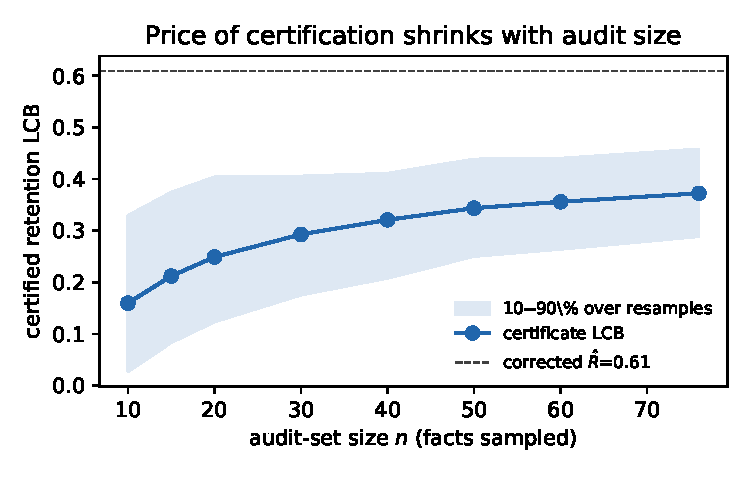
\includegraphics[width=0.31\linewidth]{figures/certify_sizing.pdf}
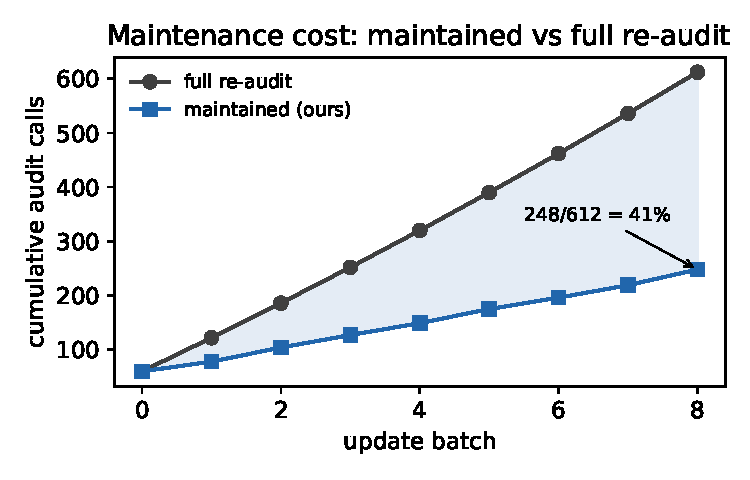
\includegraphics[width=0.31\linewidth]{figures/certify_cost.pdf}
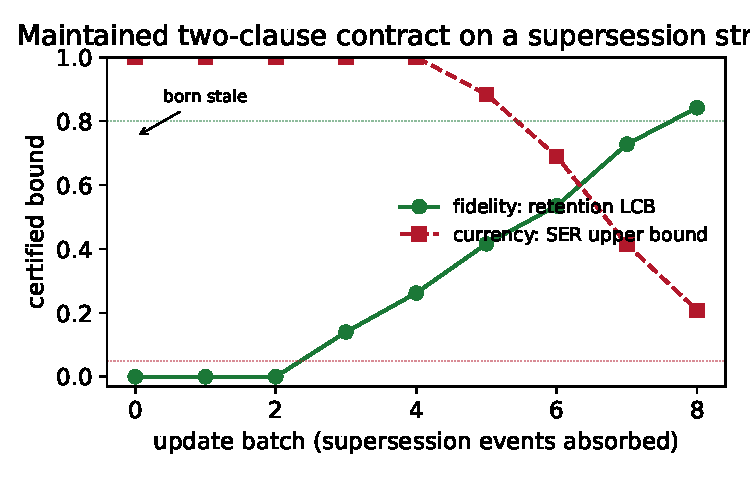
\includegraphics[width=0.31\linewidth]{figures/certify_currency.pdf}
\caption{Left: price of certification (raw estimate minus certified lower bound) vs.\ audit size $n$. Middle: maintained certificate cost vs.\ cumulative full-audit cost across churn batches. Right: maintained fidelity/currency bounds tracking a store from born-stale to current (\S\ref{sec:certify-currency}).}
\label{fig:certify-sizing}
\end{figure}

\subsection{The build lottery: certification matters because point estimates are not reproducible}
\label{sec:build-lottery}

Two independently compiled stores from the \emph{same} corpus, same compiler, same prompt, disagree with each other on $17.1$--$23.3\%$ of per-claim outcomes (measured across two corpus scales, $200$-doc/$25$-page and $400$-doc/$50$-page). One example pair: build A certifies $R \ge 0.327$ while build B's true (oracle) retention is $0.506$ --- either build alone, reported as a point estimate, would mislead in a different direction. This is the concrete justification for certifying with a confidence bound rather than reporting whichever single compile happened to run: LLM compilation is stochastic enough that ``the'' retention of a store is not well-defined without a distribution over builds.

\subsection{Maintaining the certificate as the store changes}

A certificate computed once goes stale as new documents arrive, exactly like the store it describes. We test whether the certificate can be kept valid incrementally, without a full re-audit after every update. On a healthy update stream, maintained certification matches full-audit validity at $40.5\%$ of the query cost ($248$ vs.\ $612$ calls). On an adversarial churn stream (documents arriving fast enough to threaten validity), a stale certificate (last-computed bound LCB $= 0.386$) is breached by batch $7$ as true retention falls to $0.378$; the maintained certificate tracks the decline ($0.357 \to 0.183$) and stays valid throughout, at $85\%$ of full-audit cost ($581$ vs.\ $684$ calls). The certificate is only useful if it is re-validated at the cadence the store actually changes --- a one-time audit would have silently gone stale exactly when it mattered most.

\subsection{The adaptivity trap: self-audited repair overclaims}

A natural response to a low certified score is to repair the store and re-certify. If the repair is \emph{targeted} at the same claims used to detect the problem, the resulting certificate is contaminated by the targeting: a repair-set-audited certificate reads $R = 0.760$ while an honest holdout audit of the same repaired store reads $R = 0.244$ --- a $52$-point overclaim from self-audit alone, with no change to the store's actual quality. The honest fix is not to skip repair, but to avoid auditing on the set that motivated the repair: compiling twice and taking the union of two independent compiles raises the \emph{honest} (holdout) bound from $0.244$ to $0.389$, a genuine $+0.14$ gain, at roughly double the compile cost. This distinction --- overclaiming from self-audit vs.\ a real, if smaller, gain from an honest procedure --- recurs in \S\ref{sec:maintain} as the difference between a maintainer that games its own reward signal and one that does not.

\subsection{Currency under a two-clause contract}
\label{sec:certify-currency}

Combining both clauses on HoH: a store compiled with no currency awareness starts \emph{born-stale} ($R{=}0$, $\mathrm{SER} \le 1.0$ uncertified); after maintenance under the two-clause contract, the certified bounds reach $R \ge 0.842$ and $\mathrm{SER} \le 0.208$, at $47\%$ of full-audit cost ($504$ of $1080$ calls). This is the compile-stage result of \S\ref{sec:compile} restated as a certificate rather than a point estimate: not just ``the compiled store is more current,'' but a stated, auditable confidence bound on how current, kept valid as the store keeps changing.
